\section{Finita elementmetoden}
\label{sec:femtheory}

Inom fysiken modelleras ofta fysikaliska fenomen med partiella differentialekvationer.
Dessa kan ofta vara icketriviala att evaluera analytiskt. Det finns en
rad olika metoder för att hantera sådana problem genom approximationer. En av
dessa metoder kallas finita elementmetoden. Den går ut på att den
partiella differentialekvationen eller systemet av kopplade partiella
differentialekvationer delas upp i små delar som är mer lätthanterliga.
Denna metod tillåter också evalueringen av problem vars egenskaper i
definitionsmängden är inhomogena och diskontinuerliga. Dessutom kan
problemen lösas för godtycklig geometri med godtyckliga randvillkor. Alla
dessa egenskaper gör att finita elementmetoden är ett väldigt kraftfullt redskap
vid beräkning av komplicerade problem. Denna metod kommer senare i arbetet
att användas för att räkna på värme- och luftflöden.

Den undermetod av finita element\-metoden som skall användas i denna
kandidat\-uppsats är Galerkins metod.
En finita element\-lösning med Galerkins metod kräver att problemet reduceras till
ett ekvivalent variations\-problem.
Här är $L$ differential\-operatorn
som betecknar differential\-ekvationen

\begin{equation}
\label{eq:femtheoryprob}
L(u) = 0.
\end{equation}

Här är $u = u(\mathbf{r},t)$ en funktion av de spatiala koordinaterna samt tiden.
$\Phi$ definieras sedan som rummet av alla testfunktioner $\phi$ vilka
 är kontinuerliga i
definitionsmängden $\Omega$ samt vars derivator är styckvis kontinuerliga på randen
$\Gamma$. Testfunktionerna $\phi \in \Phi$ måste även vara $L^2$-integrabla.
Variationsproblemet blir då: Sök $u\in\Phi$
som uppfyller 

\begin{equation}
\label{eq:femtheoryweak}
\int_\Omega L(u)\phi(\mathbf{r}) \mathrm{d}\Omega = 0.
\end{equation}

Det är tydligt
att alla $u$ som uppfyller $L(u) = 0$ är ortogonala mot alla
$L^2$ integrabla testfunktioner eftersom integranden då alltid kommer att vara identiskt noll.
Detta variationsproblem brukar normalt kallas för den svaga formuleringen.

Om differentialekvationen innehåller andra ordningens deriveringsoperatorer krävs en utförligare analys då vissa testfunktioner som ibland används kan inte deriveras
två gånger. Dessutom så ger kommande beräkningar oss en trevlig metod syftad
till att implementera neumannvillkor, se avnsitt~\ref{subsec:boundaryenforcement}.

Divergensteoremet i två dimensioner

\begin{equation}
\label{eq:femtheorygausstheorem}
\int_\Omega \nabla\cdot \mathbf{A} \mathrm{d}\Omega = \int_\Gamma \mathbf{A}\cdot\mathbf{n}
\mathrm{d}\Gamma
\end{equation}

med $\mathbf{A} = (uw, 0)$ eller $\mathbf{A} = (0, uw)$ ger då
\begin{equation}
\label{eq:femtheory:partint}
\int_\Omega w\frac{\partial u}{\partial x_k} \mathrm{d}\Omega +
\int_\Omega u\frac{\partial w}{\partial x_k} \mathrm{d}\Omega =
\int_\Gamma uwn_k \mathrm{d}\Gamma\mbox{,   }k=1,~2.
\end{equation}

Slutligen summeras uttrycket över alla
$k$ vilket ger

\begin{equation}
\label{eq:femtheory:green}
\int_\Omega u\Delta v \mathrm{d}\Omega =
\int_\Gamma u\nabla v\cdot\mathbf{n}\mathrm{d}\Gamma-\int_\Omega \nabla v\cdot\nabla u \mathrm{d}\Omega.
\end{equation}

Här är $w$ utbytt mot $w_i$ där $\mathbf{w} = (w_1, w_2) = \nabla v$.\cite{johnson2009}

Termer som innehåller laplaceoperatatorn kan enligt ovanstående recept utvecklas
till ekvation

\begin{equation}
\label{eq:femtheorylaplacerecepie}
\int_\Omega \phi\Delta u \mathrm{d}\Omega = -\int_\Omega \nabla\phi\nabla u \mathrm{d}\Omega +
\int_\Gamma \phi \mathbf{n}\cdot\nabla u \mathrm{d}\Gamma.
\end{equation} 

Slutligen så ansätts 

\begin{equation}
\label{eq:femtheoryansatz}
u(\mathbf{r}) \approx \sum_n u_n \phi_n(\mathbf{r})
\end{equation}

vilket stoppas
in i den svaga formuleringen i ekvation \eqref{eq:femtheoryweak}. Nu kan
konstanterna i linjärkombinationen av testfunktioner plockas ut ur integralerna
och integralerna av testfunktionerna evalueras. Genom detta så kan
sedan konstanterna lösas ut genom lösning av ekvationssystemet som
fås då man låter den fria testfunktionen löpa över alla okända noder.
För exempel på dessa beräkningar se avsnitten~\ref{sec:femconvection} och
\ref{sec:femheat}.


\subsection{Spatial diskretisering}

Lösningen av de galerkinformulerade ekvationerna kräver att en basfunktion väljs.
Ett populärt val i litteraturen är linjära triangulära element då de
är lätta att använda. Det är dock bara fantasin som begränsar valet av basfunktion
och elementgeometri.
\cite{johnson2009}\cite{lewis04}\cite{reddy93}\cite{fem50} Området den
partiella differentialekvationen skall lösas i delas upp i triangulära element.
Trianglarnas hörn blir då noder och trianglarna kallas element. Elementen ligger i ett plan vars normal kallas $\phi$. Basfunktionen bildar linjära plan från noden och $\phi=1$ ned till intillliggande elements rander i planet. Basfunktionen antar värdet noll på resten av planet.\cite{johnson2009} För att se ett exempel på hur linjära
triangulära element kan se ut i en dimension se figur \ref{fig:basefunction}.

\begin{figure}
\centering
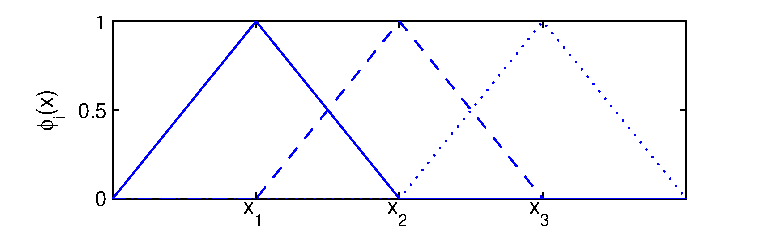
\includegraphics{images/basefunction.eps}
\caption{Illustration över basfunktionerna $\phi_1$, $\phi_2$ och $\phi_3$ i en
dimension med noderna $x_1$, $x_2$ samt $x_3$.}\label{fig:basefunction}
\end{figure}


\subsection{Påtvingande av randvillkor}
\label{subsec:boundaryenforcement}
Två typer av randvillkor är relevanta för detta arbete främst i lösning med Galerkins 
metod. Det ena är dirichletvillkor, vilket
innebär att sökt funktion antar ett visst värde på randen. Det andra är neumannvillkor,
som sätter derivatan i randnormalriktningen till ett visst värde. Tillvägagångssättet
för påtvingande av dessa villkor i Galerkins metod är lite olika. Dirichletvillkor
påtvingas lättast genom att noderna som innehar denna typ av villkor sätts till ett värde
och att ekvationerna uppdateras med detta värde. Neumannvillkor påtvingas istället
genom att värdet på dessa rander sätts in i integralerna som går över randen. Det
är viktigt att tillräckligt många randvillkor sätts. Om inte detta genomförs
så får problemet en lösning vars egenskaper inte är explicit bestämda. I värsta fall kan en en trivial lösning fås. Vilka randvillkor som väljs beror helt
på applikationen.


